% ============================================================ %
\subsection{Topologické uspořádání}
% ============================================================ %

V této části se budeme věnovat orientovaným grafům.

\noindent Představte si klasický problém každého FIŤáka před začátkem semestru. Chce si zapsat předměty, ale ty mají různé prerekvizity. Jak tedy zjistit co si zapsat může a co ne? Přesně k tomuto problému se hodí topologické uspořádání. Podobných problémů existuje celá řada. 

\noindent Může se stát, že takový problém vůbec nepůjde vyřešit? Také bychom mohli například chtít zapsat si více než jen jeden předmět, jaké si tedy může student zapsat naráz. Na všechny tyto otázky nám pomůže odpovědět následující algoritmu. Topsort. \bigskip


\begin{definition}[Topologické uspořádání]
Nechť $G = (V, E)$ je orientovaný graf. \textbf{Topologické uspořádání} grafu $G$ je takové pořadí (seřazení) jeho vrcholů $v_1, v_2, \dots, v_n$, že pro každou orientovanou hranu $(v_i, v_j) \in E$ platí $i < j$.
\end{definition}

\noindent Intuitivně, pokud nakreslíme vrcholy horizontálně do řady v pořadí topologického uspořádání zleva doprava, všechny orientované hrany (šipky) směřují výhradně zleva doprava. Tedy neexistuje šipka zpět doleva, jinak by jsme měli cyklus.

\begin{center}
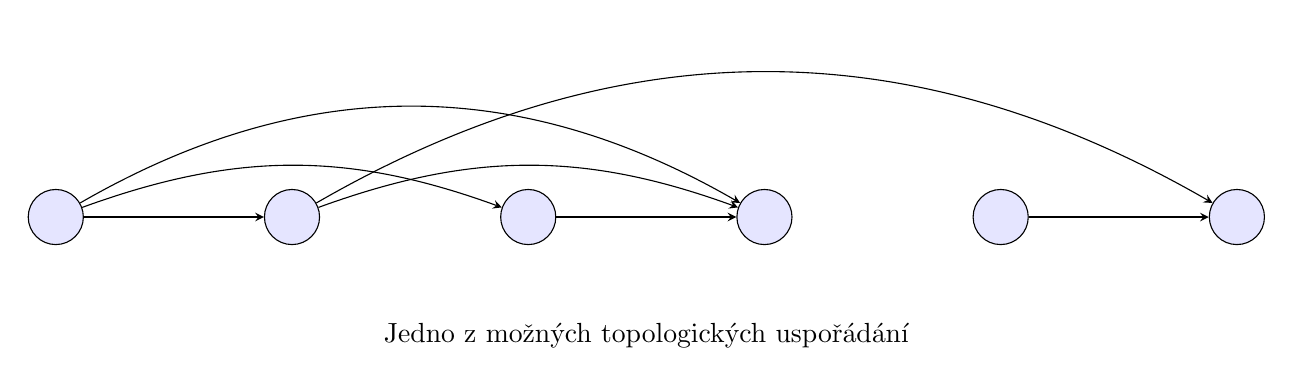
\begin{tikzpicture}[>=stealth,
    vnode/.style={circle, draw, minimum size=7mm, inner sep=0pt, fill=blue!10}]
  % Vertices placed horizontally
  \node[vnode] (a) at (0,0) {};
  \node[vnode] (b) at (3,0) {};
  \node[vnode] (c) at (6,0) {};
  \node[vnode] (d) at (9,0) {};
  \node[vnode] (e) at (12,0) {};
  \node[vnode] (f) at (15,0) {};

  % Directed edges (partial order)
  % Adjacent edges (now include all consecutive pairs)
  \draw[->] (a) -- (b);

  \draw[->] (c) -- (d);

  \draw[->] (e) -- (f);
  % Skipping edges (with bends to avoid intermediate vertices)
  \draw[->, bend left=20] (a) to (c);
  \draw[->, bend left=20] (b) to (d);
  \draw[->, bend left=30] (a) to (d);
  \draw[->, bend left=30] (b) to (f);

  % Topological ordering annotation centered below
  % Centered annotation below the whole diagram
  \node[align=center] at (7.5,-1.5) {Jedno z možných topologických uspořádání};
\end{tikzpicture}
\end{center}


\begin{definition}
Nechť $n \geq 1$. Orientovaná kružnice délky $n$ (s $n$ vrcholy) je orientovaný graf $G = (\{1, \dots , n\}, \{(i, i + 1)$ | $i \in \{1, \dots , n - 1\}\} \cup \{(n, 1)\})$.
\end{definition} \medskip

\begin{center}
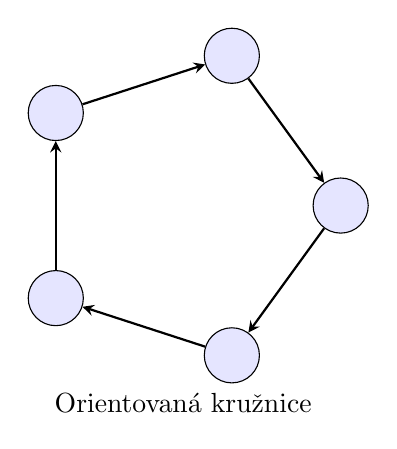
\begin{tikzpicture}[>=stealth, node distance=2cm,
    vnode/.style={circle, draw, minimum size=7mm, inner sep=0pt, fill=blue!10}]
  % Place 5 vertices on a circle without labels
  \foreach \i/\label in {0/A,1/B,2/C,3/D,4/E}{
    \node[vnode] (\label) at ({360/5*\i}:2) {};
  }
  % Draw directed edges forming a cycle
  \foreach \i/\j in {A/B,B/C,C/D,D/E,E/A}{
    \draw[<-, thick] (\i) -- (\j);
  }
  % Centered caption below the diagram
  \node[align=center] at (0,-2.5) {Orientovaná kružnice};
\end{tikzpicture}
\end{center}


\begin{definition}[Orientovaný acyklický graf]
Orientovaný graf $G$ nazveme \textbf{acyklickým}, pokud neobsahuje žádnou orientovanou kružnici.
\end{definition}

\medskip

\begin{remark}
    Těmto grafů se často říká (i v české terminologii) DAG, neboli Directed Acylic Graph.
\end{remark} 

\medskip

\noindent Pokud byste takové topologické uspořádání měli vyrobit, začli byste asi tím, že byste se snažili najít vrchol, do kterého nevede žádná hrana. Takovému vrcholu budeme říkat zdroj.

\medskip

\begin{definition}[Zdroj a stok]
Nechť $G = (V, E)$ je orientovaný graf.
\begin{itemize}
    \item Vrchol $v \in V$ nazveme \textbf{zdrojem}, pokud do něj nevede žádná orientovaná hrana.
    \item Vrchol $v \in V$ nazveme \textbf{stokem}, pokud z něj nevede žádná orientovaná hrana.
\end{itemize}
\end{definition}

\medskip

\noindent Ale musí takový vrchol existovat? Jak ho algoritmicky najít?

\medskip

\begin{theorem}[O existenci zdroje a stoku]
Nechť $G = (V, E)$ je orientovaný acyklický graf. Potom $G$ obsahuje alespoň jeden zdroj a alespoň jeden stok.
\end{theorem}

\begin{proof}
Dokážeme sporem pro zdroj (pro stok je důkaz analogický).
\begin{itemize}
    \item Předpokládejme, že v DAGu $G$ neexistuje žádný zdroj.
    
    \item Zvolme libovolný vrchol $v_1 \in V$. Jelikož $v_1$ není zdroj, vede do něj alespoň jedna orientovaná hrana z nějakého vrcholu $v_2$. Jelikož ani $v_2$ není zdroj, vede do něj hrana z $v_3$, atd.

    \item Tímto způsobem vytváříme posloupnost vrcholů $v_1, v_2, v_3, \dots$. Protože množina vrcholů $V$ je konečná ($|V| = n$), musí se nejpozději po $n + 1$ krocích dle holubníkového principu nějaký vrchol zopakovat (nechť $v_i = v_j$ pro $i < j$).

    \item Posloupnost $v_i, v_{i+1}, \dots, v_j = v_i$ však tvoří v $G$ orientovaný cyklus, což je spor s tím, že $G$ je acyklický. Tedy v $G$ musí existovat alespoň jeden zdroj.

\end{itemize}
\end{proof}

\subsubsection{Algoritmus TopSort}

Existence zdroje nám dává cestu pro sestrojení algoritmu. V každém kroku nalezneme zdroj, zpracujeme ho a odebereme z orientovaného grafu $G$. Takto vyrobíme topologické uspořádání grafu $G$. Pokud bychom v nějakém kroku nebyli schopni nalézt zdroj grafu, pak díky větě o existenci zdroje, musí nutně obsahovat cyklus a topologické uspořádání nelze nalézt.\bigskip

\noindent Jak funguje topsort: Spočítáme si vstupní stupně pro každý vrchol $v$ (tedy počet hran co vedou \textbf{do} vrcholu $v$). Do fronty dáme vrcholy se vstupním stupněm 0, ty jsou zdroji v počátečním grafu. Vždy při odebrání zdroje $z$ s ním odebereme i jeho hrany a každému \textbf{následníkovi} snížíme stupeň o jedna. Pokud tomuto následníkovi klesne stupeň na 0, pak se stává zdrojem a my ho přidáme do fronty. \medskip

\noindent\textbf{Vstup}: Orientovaný graf $G = (V, E)$. \\
\noindent\textbf{Výstup}: Topologické uspořádání vrcholů $G$, nebo hlášení, že graf obsahuje cyklus. \\
\funkce{TopSort}{orientovaný graf $G$}
\begin{pseudocode}
\item $Q := \text{prázdná fronta}$
\item Pro každý vrchol $v \in V(G)$: $\delta[v] := 0$ \textcolor{gray}{// Pole vstupních stupňů}
\item Pro každou hranu $(u, v) \in E(G)$: $\delta[v] := \delta[v] + 1$
\item Vlož do $Q$ všechny vrcholy $z \in V(G)$ splňující $\delta[z] = 0$
\item Dokud fronta $Q$ není prázdná:
\item \tab Vyjmi prvek $z$ ze začátku fronty $Q$
\item \tab Vypiš $z$ \textcolor{gray}{// Přidej $z$ na další pozici topologického uspořádání}
\item \tab Pro každou orientovanou hranu $(z, w)$ vedoucí z $z$:
\item \tab \tab $\delta[w] := \delta[w] - 1$
\item \tab \tab Pokud $\delta[w] = 0$: zařaď $w$ na konec fronty $Q$
\item Pokud nebyly zpracovány všechny vrcholy grafu $G$:
\item \tab Graf $G$ obsahuje orientovaný cyklus!
\end{pseudocode} 

\bigskip

\begin{theorem}[O správnosti algoritmu TopSort]
Algoritmus $\text{TopSort}(G)$ doběhne v konečném čase a buď vygeneruje platné topologické uspořádání, nebo správně detekuje orientovaný cyklus.
\end{theorem}

\medskip

\begin{proof}
Vstupní stupeň $\delta[v]$ udává počet dosud neodebraných předchůdců vrcholu $v$.
Vrchol $v$ je vložen do fronty $Q$ právě tehdy, když vstupní $\delta[v] = 0$, tedy až poté, co byli všichni jeho předchůdci vyjmuti a vypisováni. Proto pro každou hranu $(u, v) \in E$ bude $u$ vypsán dříve než $v$, což zaručuje korektnost výstupního pořadí. \\
Pokud graf obsahuje orientovaný cyklus $C$, žádný vrchol $v \in C$ nemůže nikdy dosáhnout $\delta[v] = 0$, protože má předchůdce na cyklu. Fronta $Q$ se vyprázdní dříve, než budou zpracovány všechny vrcholy, a algoritmus na řádku (12) správně zahlásí cyklus.
\end{proof} \bigskip

\begin{theorem}[O složitosti algoritmu TopSort]
Při reprezentaci orientovaného grafu $G = (V, E)$ seznamem následníků má algoritmus $\text{TopSort}$ časovou i paměťovou složitost $\bigO{|V| + |E|}$.
\end{theorem}

\begin{proof}
Inicializace a výpočet vstupních stupňů trvá $\bigTheta{|E|}$. Každý vrchol je do fronty $Q$ vložen a vyjmut nejvýše jednou ($\bigO{|V|}$). Každá hrana je prohledána přesně jednou při odebrání svého počátečního vrcholu ($\bigO{|E|}$). Celková časová složitost je tedy $\bigO{|V| + |E|}$. Graf $G$, pole $\delta$ a fronta $Q$ zaberou nejvýše $\bigO{|V| + |E|}$ paměti.
\end{proof}
